% chktex-file 13
% chktex-file 18
% chktex-file 44

\documentclass[a4paper, 12pt]{article}
\usepackage{algorithm}
\usepackage{algpseudocode}
\usepackage{amsfonts}

\usepackage{amsmath}
\usepackage[french]{babel}
\usepackage{dirtree}
\usepackage{enumitem}
\usepackage[T1]{fontenc}
\usepackage{geometry}
\geometry{hmargin=2cm,vmargin=1.9cm}
\usepackage{graphicx} % Required for inserting images
\usepackage{hyperref}
\usepackage{mathtools}
\usepackage{spverbatim}

\title{LEPL1503 --- Projet 3 \\ Opérations sur les matrices}
\author{Charles Van Hees \and Matthieu Pigaglio \and Olivier Bonaventure \and Benoît Legat}
\date{Année académique 2024~--~2025}

\begin{document}
\maketitle

Les matrices sont omniprésentes dans le monde de l'ingénierie et de l'informatique. Que ce soit pour faire des sciences des données ou des éléments finis, cet objet mathématique est souvent manipulé dans des programmes informatiques. Au cours de ce projet, vous apprendrez à utiliser efficacement les matrices avec le langage C. Vous développerez des algorithmes efficaces pour réaliser des opérations élémentaires sur les vecteurs et matrices. L'objectif de ce projet est d'apprendre la programmation avec le langage C et, en moindre mesure, l'algorithmique.

\section{Le projet}
\noindent Nous vous demandons de coder efficacement plusieurs opérations sur les matrices. Celles-ci ont été réparties en plusieurs groupes~:
\begin{enumerate}
    \item Les opérations basiques sont~: 
    \begin{enumerate}
        \item l'addition de 
        \begin{itemize}
            \item deux vecteurs (add\_v\_v)
            \item et de deux matrices (add\_m\_m),
        \end{itemize}
        \item la soustraction de
        \begin{itemize}
            \item deux vecteurs (sub\_v\_v) 
            \item et de deux matrices (sub\_m\_m)
        \end{itemize}
        \item le produit scalaire entre deux vecteurs (dot\_prod),
        \item la norme d'un vecteur (norm),
        \item la multiplication entre une matrice et un vecteur (mult\_m\_v)
        \item et entre deux matrices (mult\_m\_m),
        \item et la transposée d'une matrice (transp).
    \end{enumerate}  
    Cette partie est obligatoire~! Vous trouverez dans l'annexe~\ref{app:basic_op} des schémas expliquant ces neuf opérations~;
    \item La substitution arrière (back\_sub), expliquée dans l'annexe~\ref{app:back_sub}~;
    \item La décomposition QR d'une matrice (qr). Cette partie étant plus compliquée, l'annexe~\ref{app:qr} présente en détail son fonctionnement~;
    \item Enfin, il vous est proposé de mettre à profit tout votre travail en réalisant une application de la décomposition QR~: une régression polynomiale au sens des moindres carrés (lstsq). Cette dernière partie fera intervenir toutes les parties précédents. Les détails sont fournis dans l'annexe~\ref{app:lq}.
\end{enumerate}

\noindent Ce projet se déroulera en trois étapes, entremélées avec les séances d'apprentissage du C.

\subsection*{Etape 1 - Version séquentielle du projet}
Dans un premier temps, vous allez écrire une version séquentielle du projet. Un squelette vous est fourni. Prenez tout d'abord le temps de bien comprendre tout ce qui est déjà implémenté. Pour vous aider dans votre travail, les opérations d'addition de deux vecteurs et de deux matrices sont déjà faites. 

Cependant, une fuite de mémoire s'est glissée dans le code. Après avoir lu, compris et corrigé cette erreur, vous pouvez coder les différentes opérations ci-dessus. 

Il existe plusieurs méthodes pour réaliser ces opérations, notamment pour la décomposition QR d'une matrice. Vous êtes libres de choisir celle que vous préférez\footnote{Si vous désirez utiliser d'autres algorithmes que ceux présentés dans les annexes, veillez à ce qu'ils soient stables numériquement. Bien que certains algorithmes sont mathématiquement corrects, ils peuvent mener à des résultats numériques très surprenant.}. Notez que seule l'exactitude des fichiers de sortie sera vérifiée. Vous pouvez donc coder ces opérations de la façon que vous voulez, tant que le fichier de sortie est correct (et qu'il n'y a pas de fuite de mémoire)\footnote{Il peut être intéressant d'utiliser des algorithmes en place pour diminuer la consommation mémoire. Pensez à aller voir ce que ça veut dire.}. 

Des améliorations peuvent ainsi être apportées au squelette qui vous est fourni pour diminuer son temps d'exécution et/ou sa consommation mémoire.

\subsection*{Etape 2 - Les fichiers}
Après avoir vu les fichiers, vous pourrez implémenter la lecture et l'écriture de fichiers. Ces deux premières étapes feront l'objet d'une évaluation intermédiaire.

\subsection*{Etape 3 - Version multithreadée du projet}
Enfin, vous devrez réaliser une version multithreadée du projet. Le nombre de threads sera fourni en argument au programme. Vous testerez cette version sur un Raspberry Pi avec quatre cœurs. Le multithreading devrait vous permettre de diminuer le temps d'exécution, mais également d'améliorer la consommation mémoire de votre programme. Vous ne devez paralléliser que les opérations basiques sur des matrices. En effet, la substitution arrière et la décomposition QR se prêtent moins à la parallélisation, bien qu'il soit possible d'obtenir de légers gains. Si vous voulez aller plus loin, vous pouvez essayer de paralléliser ces opérations, et de commenter les résultats que vous obtiendrez.
\subsection*{Egalement à rendre}
\paragraph{Tests} À côté de ces trois parties, il vous est demandé d'écrire des tests pour montrer que votre code fonctionne. Ceux-ci devront être réalisés avec la librairie CUnit. Des exemples de tests vous sont fournis pour les fonctions \texttt{add\_v\_v} et \texttt{add\_m\_m}.

\paragraph{README} Pour un lecteur qui n'a pas travaillé sur le projet, il est parfois difficile de se plonger dedans. Ainsi, nous vous demandons d'écrire un README expliquant la structure de votre projet et la façon de l'utiliser.

\paragraph{Makefile} Vous devrez compléter le Makefile fourni. Le code doit au minimum être compilé avec les flags \texttt{-Wall} et \texttt{-Werror} de \texttt{clang}. Le Makefile doit contenir au moins trois cibles~:
\begin{itemize}[leftmargin=0cm]
    \item \texttt{make}~: compile le programme et produit l'exécutable nommé \texttt{main}, à la racine du répertoire~;
    \item \texttt{make tests}~: compile le programme et lance les tests que vous avez écrits~;
    \item \texttt{make clean}~: nettoie le projet en supprimant l'exécutable et les fichiers objets produits lors de la compilation.
\end{itemize}

\paragraph{Rapport} Finalement, il vous est demandé d'écrire un rapport de maximum cinq pages. Dans celui-ci, vous présenterez les algorithmes que vous avez implémentés et les améliorations que vous avez apportées. Il n'est pas nécessaire de réécrire les algorithmes des annexes. Cependant, si vous utilisez d'autres algorithmes, il peut être intéressant de les expliquer et de justifier vos choix. Vous décrirez également brièvement les tests unitaires que vous avez produits. Enfin, vous réaliserez une analyse détaillée des performances de votre projet en utilisant le Raspberry Pi. Il vous est demandé d'analyser les trois métriques de performance suivantes~: le temps d'exécution, la consommation mémoire et la consommation énergétique. Cette analyse contiendra une comparaison en fonction du nombre de threads. N'oubliez pas d'ajouter une bibliographie.

\section{Détails pratiques}
\paragraph{Spécifications du programme}
Le Makefile génère un exécutable \texttt{main}. Vous pouvez l'utiliser de la façon suivante~:
\begin{spverbatim}
./main name_op input_file_A [-v] [-n n_threads] [-f output_stream] 
                                            [-d degree] [input_file_B]
\end{spverbatim}
\noindent Les crochets indiquent que l'argument est optionnel. Les noms des opérations sont ceux repris entre parenthèses à côté des noms complets dans la section précédente. Toutes les opérations nécessitent deux fichiers d'instance, excéptés norm, transp et qr. C'est via cette commande que nous testerons votre programme. Seul le fichier de sortie sera pris en compte pour vérifier l'exactitude de votre code.

\noindent Vous trouverez des détails sur les arguments en utilisant la commande
\begin{verbatim}
    ./main -h
\end{verbatim}

\paragraph{Format d'un fichier}
Les fichiers seront au format binaire. Leur contenu dépend de ce que doit réaliser l'opération.\\
Si le résultat d'une fonction est un double, le fichier ne contiendra que ce dernier.\\
Pour ce qui est des vecteurs (que ce soit pour un fichier d'entrée ou de sortie), le fichier contient dans l'ordre les valeurs suivantes~:
\begin{itemize}
    \item La taille $m$ du vecteur. Cette valeur est un entier non-signé encodé sur 64 bits en big-endian. Comme expliqué dans le \href{https://sites.uclouvain.be/SyllabusC/notes/Theorie/Fichiers/fichiers.html\#utilisation-des-fichiers}{syllabus}, les entiers ne sont pas représentés de la même façon sur tous les ordinateurs. Les fonctions \texttt{htobe64} et \texttt{be64toh} vous seront utiles~;
    \item Toutes les valeurs contenues dans le vecteur dans l'ordre (donc d'abord celle à l'indice $0$, puis celle à l'indice $1$\dots). Les valeurs contenues dans les vecteurs sont des double.
\end{itemize}
Pour ce qui est des matrices (entrée ou sortie), le fichier contient~:
\begin{itemize}
    \item Le nombre de lignes $m$ de la matrice (entier non-signé encodé sur 64 bits en big-endian)~;
    \item Le nombre de colonnes $n$ de la matrice (entier non-signé encodé sur 64 bits en big-endian). Notons que si $m$ est nul, alors $n$ est nul et inversément~;
    \item Les lignes de la matrice. Chaque ligne commence par un uint64\_t (en big-endian) indiquant le numéro de la ligne, et est suivi des $n$ valeurs (double) de cette ligne.
\end{itemize}
Enfin, pour la décomposition QR, le fichier de sortie contiendra~:
\begin{itemize}
    \item Le nombre de lignes $m$ de la matrice $Q$ (entier non-signé encodé sur 64 bits en big-endian)~;
    \item Le nombre de colonnes $n$ de $Q$ (entier non-signé encodé sur 64 bits en big-endian)~;
    \item Les valeurs de la matrice Q, comme pour une simple matrice (ligne par ligne)~;
    \item Les valeurs de la matrice R, comme pour une simple matrice (ligne par ligne).
\end{itemize}

\paragraph{Avant d'avoir vu les fichiers} Comme vous n'aurez pas vu les fichiers au moment de commencer le projet, nous vous fournissons un fichier objet \texttt{file.o} dans le dossier \texttt{objects}. Son utilisation vous permettra de lire et d'écrire des fichiers en utilisant les fonctions fournies dans le fichier header correspondant, comme réalisé actuellement pour les opérations add\_v\_v et add\_m\_m. Cependant, vous devrez coder ces fonctions plus tard et ceci sera vérifié~!

\paragraph{Arborescence}
Il vous est demandé de respecter scrupuleusement l'arborescence ci-dessous. Des tests automatiques seront réalisés. Si l'arborescence n'est pas respectée, ceux-ci échoueront. N'ajoutez pas de dossiers/fichiers inutiles dans votre soumission~! (par exemple, pas de dossier \texttt{help})
\dirtree{%
    .1 /.
    .2 headers \qquad Ce dossier contient les fichiers headers (.h).
    .2 src     \qquad \qquad Ce dossier contient les fichiers sources (.c).
    .2 tests   \qquad \quad Ce dossier contient les codes des tests.
    .2 Makefile.
    .2 rapport\_groupe\_A1.pdf.
    .2 README.
}

\noindent L'exécutable doit porter le nom \texttt{main} et se trouver à la racine du dossier.

\paragraph{Pour vous aider} Nous mettons à votre disposition dans le dossier \texttt{help} des codes pour générer des fichiers contenant des vecteurs et des matrices. Vous pouvez écrire votre vecteur ou matrice et donner le nom du fichier dans lequel vous voulez qu'il soit stocké. Ensuite, utilisez les commande \texttt{make generator\_vector} ou \texttt{make generator\_matrix} pour obtenir le fichier binaire contenant la matrice.

\paragraph{Échéancier} Vous trouverez ci-dessous l'ensemble des échéances.
\begin{table}[!htb]
\centering
    \begin{tabular}{|c|c|}
        \hline
            & Date\\
        \hline
        Rendu pour Peer review  & 28/03/2025\\
        \hline
        Rendu final & 12/05/2025\\
        \hline
        Oral & 19/05/2025\\
        \hline
    \end{tabular}
\end{table}

\begin{itemize}
    \item \textbf{Rendu pour Peer review:} Vous rendrez un code ainsi qu'un readme expliquant comment lancer votre code ainsi que les éventuels bug de votre code. 
    \item \textbf{Rendu final:} Vous fournirez votre code ainsi qu'un readme expliquant votre suite de test. \textbf{Vérifiez avant de rendre que vos solutions passent bien les tests disponibles sur Inginious. La cotation prend en compte le passage de ces tests ainsi que des tests supplémentaires sur la qualité de code et la non présence de fuite de mémoires.}
    \item \textbf{Oral:} Durant cet oral, il vous sera demander d'expliquer entièrement votre code.
\end{itemize}

\appendix
\section{Opérations basiques}\label{app:basic_op}
\noindent Vous trouverez ci-dessous des illustrations des opérations basiques.
\paragraph{Addition de deux vecteurs (add\_v\_v)}
Cette fonction prend en entrée deux vecteurs de même dimension et sort un vecteur de même dimension. Exemple~:
\begin{equation*}
      \begin{pmatrix} 1 &  2 & 3 \end{pmatrix}
    + \begin{pmatrix} 3 & -2 & 0 \end{pmatrix}
    = \begin{pmatrix} 4 &  0 & 3 \end{pmatrix}
\end{equation*}

\paragraph{Addition de deux matrices (add\_m\_m)}
Cette fonction prend en entrée deux matrices de mêmes dimensions et sort une matrice de mêmes dimensions. Exemple~:
\begin{equation*}
      \begin{pmatrix} 1 &  2 & 3 \\ 4 &  5 & 6   \end{pmatrix}
    + \begin{pmatrix} 3 & -2 & 0 \\ 3 & -7 & 0.2 \end{pmatrix}
    = \begin{pmatrix} 4 &  0 & 3 \\ 7 & -2 & 6.2 \end{pmatrix}
\end{equation*}

\paragraph{Soustraction de deux vecteurs (sub\_v\_v)}
Cette fonction prend en entrée deux vecteurs de même dimension et sort un vecteur de même dimension. Exemple~:
\begin{equation*}
      \begin{pmatrix} 1  &  2 & 3 \end{pmatrix}
    - \begin{pmatrix} 3  & -2 & 0 \end{pmatrix}
    = \begin{pmatrix} -2 &  4 & 3 \end{pmatrix}
\end{equation*}

\paragraph{Soustraction de deux matrices (sub\_m\_m)}
Cette fonction prend en entrée deux matrices de mêmes dimensions et sort une matrice de mêmes dimensions. Exemple~:
\begin{equation*}
      \begin{pmatrix} 1  &  2 & 3 \\ 4 &  5 & 6   \end{pmatrix}
    - \begin{pmatrix} 3  & -2 & 0 \\ 3 & -7 & 0.2 \end{pmatrix}
    = \begin{pmatrix} -2 &  4 & 3 \\ 1 & 12 & 5.8 \end{pmatrix}
\end{equation*}

\paragraph{Produit scalaire entre deux vecteurs (dot\_prod)}
Cette fonction prend en entrée deux vecteurs de même dimension et sort un double. Exemple~:
\begin{equation*}
        \begin{pmatrix} 1  &  2 & 3 \end{pmatrix}
  \cdot \begin{pmatrix} 3  & -2 & 0 \end{pmatrix}
  =     1 \cdot 3 + 2 \cdot -2 + 3 \cdot 0 = -1
\end{equation*}

\paragraph{Norme euclidienne d'un vecteur (norm)}
Cette fonction prend en entrée un vecteur et sort un double. Exemple~:
\begin{equation*}
    \lVert \begin{pmatrix} 3 & 4 \end{pmatrix} \rVert
  = \sqrt{3 \cdot 3 + 4 \cdot 4} = 5
\end{equation*}

\paragraph{Multiplication d'une matrice avec un vecteur (mult\_m\_v)}
Cette fonction prend en entrée une matrice de dimensions $m \times n$ et un vecteur de dimension $n$ et sort un vecteur de dimension $m$. Exemple~:
\begin{equation*}
          \begin{pmatrix} 1  &  2 & 3 \\ 4 &  5 & 6   \end{pmatrix}
    \cdot \begin{pmatrix} 3  \\ -2 \\ 0 \end{pmatrix}
    =     \begin{pmatrix} -1 \\ 2 \end{pmatrix}
\end{equation*}

\paragraph{Multiplication de deux matrices (mult\_m\_m)}
Cette fonction prend en entrée une matrice de dimensions $m \times n$ et une matrice de dimensions $n \times p$ et sort une matrice de dimensions $m \times p$. Exemple~:
\begin{equation*}
          \begin{pmatrix} 1  &  2 \\ 4 &  5   \end{pmatrix}
    \cdot \begin{pmatrix} 3  & -2 & 0 \\ -2 &  1 & 2  \end{pmatrix}
    =     \begin{pmatrix} -1 &  0 & 4 \\  2 & -3 & 10 \end{pmatrix}
\end{equation*}

\paragraph{Transposée d'une matrice (transp)}
Cette fonction prend en entrée une matrice de dimensions $m \times n$ et sort une matrice de dimensions $n \times m$. Exemple~:
\begin{equation*}
     {\begin{pmatrix} 3  & -2 & 0 \\ -2 &  1 & 2   \end{pmatrix}}^T
    = \begin{pmatrix} 3  & -2 \\ -2 &  1 \\ 0 & 2  \end{pmatrix}
\end{equation*}

\newpage
\section{Substitution arrière}\label{app:back_sub}
La substitution arrère est utilisée pour résoudre un système $Ux = b$, avec $U$ une matrice carrée triangulaire supérieure (avec des zéros en dessous de la diagonale principale) et $b$ un vecteur. On parle de substitution arrière car sa résolution commence par la dernière ligne et remonte petit à petit. Considérons le système suivant~:
\begin{equation*}
          \begin{pmatrix} 1 & 2 \\ 0 & 3 \end{pmatrix}
    \cdot \begin{pmatrix} x_1   \\ x_2   \end{pmatrix}
    =     \begin{pmatrix} 5     \\ 3     \end{pmatrix}
\end{equation*}
Pour le résoudre, on commence par la fin en trouvant la valeur de $x_2$. La dernière équation donne $3 x_2 = 3$. On en déduit que $x_2 = 1$. Ensuite, il est possible de trouver la valeur de $x_1$ via l'équation au-dessus~:
\begin{align*}
                    x_1 + 2       x_2 &= 5 \\
    \Leftrightarrow x_1 + 2 \cdot 1   &= 5 \\
    \Leftrightarrow x_1               &= 3
\end{align*}

\paragraph{Algorithme} L'algorithme~\ref{alg:back_sub} présente la substitution arrière.

\begin{algorithm}[!htb]
    \caption{Substitution arrière}\label{alg:back_sub}
    \begin{algorithmic}[1]
        \Require{$U \in {\mathbb{R}}^{m \times m}$ est une matrice triangulaire supérieure}
        \Require{$b \in {\mathbb{R}}^{m}$}
        \State{$x=b$}
        \For{$i$ in $m, \dots, 1$}
            \For{$j$ in $m, \dots, i+1$}
                \State{$x[i] -= A[i][j] * x[j]$}
            \EndFor{}
            \State{$x[i] /= A[i][i]$}\label{back_sub:zero}
        \EndFor{}
    \end{algorithmic}
\end{algorithm}

Nous vous demandons également de traiter les cas particuliers. Ceux-ci ont lieu lorsque $A[i][i] == 0$ (dans quel cas une division par $0$ a lieu à la ligne~\ref{back_sub:zero}). Deux situations sont possibles~:
\begin{itemize}[leftmargin=0cm]
    \item Soit $x[i] != 0$, dans quel cas le système est impossible. Dans ce cas, vous devez imprimer sur la sortie d'erreur standard le message "Aucune solution" et le programme doit se terminer avec une erreur. Le fichier de sortie n'a pas besoin d'être créé.
    \item Soit $x[i] == 0$, dans quel cas le système peut posséder une infinité de solutions. Vous pouvez continuer l'algorithme en plaçant une valeur de votre choix ou aléatoire dans $x[i]$. Si l'algorithme se termine sans erreur, imprimez le messsage "Infinité de solutions" sur la sortie d'erreur standard, et achevez le programme avec succès.
\end{itemize}

\noindent Le calcul en virgule flottante n'étant pas parfaitement précis, vous pouvez considérer qu'une valeur est nulle si celle-ci a une valeur absolue inférieure à \texttt{DBL\_EPSILON} définie dans la librairie \texttt{float.h}. Par ailleurs, pour des matrices aléatoires, limitez-vous à des dimensions de 100 environ pour vos tests pour éviter tout soucis.

\newpage
\section{Décomposition QR}\label{app:qr}
Soit $A \in {\mathbb{R}}^{m \times n}$, avec $m \geq n$ (nous ne considérons pas le cas avec $n > m$ par simplicité). La décomposition QR de cette matrice consiste à écrire $A = QR$ avec $Q \in {\mathbb{R}}^{m \times n}$ une matrice ayant des colonnes orthogonales et $R \in {\mathbb{R}}^{n \times n}$ une matrice triangulaire supérieure. Dire que $Q$ a des colonnes orthogonales signifie que $Q^T Q = {Id}_{n}$ avec ${Id}_{n}$ la matrice identité de taille $n$.

\paragraph{Algorithme} Pour réaliser cette décomposition QR, nous allons utiliser l'algorithme de Gram-Schmidt. Il en existe d'autres, vous êtes libres de les explorer.

\begin{algorithm}[!htb]
    \caption{Algorithme de Gram-Schmidt}\label{alg:gram_schmidt}
    \begin{algorithmic}[1]
        \Require{$A \in {\mathbb{R}}^{m \times n}$ avec $m \geq n$}
        \State{$Q = A$}
        \State{$R = 0$}
        \For{$i$ in $1, \dots, n$}
            \State{$R[i,i] = norm(Q[:,i])$}
            \State{$Q[:,i] /= R[i,i]$}\label{qr:zero}
            \For{$j$ in $i+1, \dots, n$}
                \State{$R[i,j] = dot\_prod(Q[:,i], Q[:,j])$}
                \State{$Q[:,j] -= R[i,j] * Q[:,i]$} \Comment{On enlève la composante parallèle à $Q[:,i]$}
            \EndFor{}
        \EndFor{}
    \end{algorithmic}
\end{algorithm}
À nouveau, il vous faut traiter les exceptions, qui auront lieu si $R[i,i] == 0$. Cela signifie que $Q[:,i]$ est une combinaison linéaire des colonnes précédentes de la matrice. Dans ce cas, la ligne~\ref{qr:zero} doit être remplacée par l'algorithme~\ref{alg:defficient}.

\begin{algorithm}[!htb]
    \caption{Cas d'une matrice défficiente}\label{alg:defficient}
    \begin{algorithmic}[1]
        \State{$Q[:,i] = $ vecteur aléatoire de taile $m$}
        \For{$j$ in $1, \dots, i-1$}
            \State{$Q[:,i] -= dot\_prod(Q[:,j], Q[:,i]) * Q[:,j]$}
        \EndFor{}
        \If{$norm(Q[:,i] == 0)$} restart
        \Else{}
            \State{$Q[:,i] /= norm(Q[:,i])$}
            \State{continue}
        \EndIf{}
    \end{algorithmic}
\end{algorithm}

\noindent Le calcul en virgule flottante n'étant pas parfaitement précis, vous pouvez considérer qu'une valeur est nulle si celle-ci a une valeur absolue inférieure à \texttt{DBL\_EPSILON} définie dans la librairie \texttt{float.h}.

\newpage

\section{Régression polynomiale au sens des moindres carrés}\label{app:lq}
La décomposition d'une matrice sous sa forme QR peut être très utile pour résoudre efficacement un système d'équations linéaires surdéterminé. Considérons le système $Ax = b$, avec $A \in {\mathbb{R}}^{m \times n}$, $m \geq n$, et $b \in {\mathbb{R}}^{m}$. Supposons en outre que $A$ soit de rang plein (cela signifie que toutes ses colonnes sont linéairement indépendantes). Si ce système n'admet pas de solution, les équations normales~\ref{eq:normal_eq} fournissent une solution approchée au système.
\begin{equation}
    A^T A x = A^T b \label{eq:normal_eq}
\end{equation}
Ces équations peuvent être résolues très facilement en utilisant la décomposition QR de $A$~!
\begin{align*}
                    A^T     A   x &= A^T     b \\
    \Leftrightarrow R^T Q^T Q R x &= R^T Q^T b \\
    \Leftrightarrow R^T       R x &= R^T Q^T b \\
    \Leftrightarrow           R x &=     Q^T b
\end{align*}

\noindent Finalement, l'algorithme~\ref{alg:lq} fait le travail, et ce en très peu de lignes.

\begin{algorithm}
    \caption{Résolution d'un système linéaire surdéterminé}\label{alg:lq}
    \begin{algorithmic}[1]
        \Require{$A \in {\mathbb{R}}^{m \times n}$, avec $m \geq n$}
        \Require{$b \in {\mathbb{R}}^{m}$}
        \State{$Q$, $R$ $\leftarrow$ QR$(A)$}
        \State{$\tilde{b} = Q^T b$}
        \State{$back\_sub(R, \tilde{b})$}
    \end{algorithmic}
\end{algorithm}

Pour aller plus loin, vous pouvez réfléchir théoriquement aux avantages de cet algorithme comparé à un algorithme basique qui consisterait simplement à résoudre le système d'équations normales (via l'élimination gaussienne par exemple). Pour les plus motivés, vous pouvez également coder l'élimination gaussienne et faire des expériences numériques.

\noindent Ceci peut être utilisé pour réaliser une approximation polynomiale au sens des moindres carrés. Supposons que nous disposons de $m$ points dans le plan $(X_i, Y_i)$. Nous souhaitons trouver un polynôme d'ordre $n$ (inférieur à $m$) qui passe au plus proche de ces points~:
\begin{equation*}
    p(x) = \sum_{j=0}^{n} a_j x^j
\end{equation*}

\noindent Dans l'idéal, Ce polynôme passe exactement par tous les points~:
\begin{equation*}
    Y_i = \sum_{j=0}^{n} a_j X_i^j \qquad i = 0, \dots, m-1
\end{equation*}
Ceci peut être réécrit sous la forme d'un système matriciel~:
\begin{equation*}
    \begin{pmatrix} X_0^0 & X_0^1 & \cdots & X_0^n \\
                    X_1^0 & X_1^1 & \cdots & X_1^n \\
                    \vdots & \vdots & \ddots & \vdots \\
                    X_{m-1}^0 & X_{m-1}^1 & \cdots & X_{m-1}^n
    \end{pmatrix}
    \cdot
    \begin{pmatrix} a_0 \\ \vdots \\ a_n \end{pmatrix}
    =
    \begin{pmatrix} Y_0 \\ Y_1 \\ \vdots \\ Y_{m-1} \end{pmatrix}
\end{equation*}

\noindent En général, nous souhaitons faire une approximation de degré faible, avec donc $n << m$. Nous faisons alors face à un problème surdimensionné qui peut être résolu avec l'algorithme~\ref{alg:lq}. Notons que cette méthode ne sera pas idéale pour des approximations de degré trop élevé.

\noindent Pour synthétiser, vous devez dans un premier temps créer la matrice A et dans un second temps appliquer l'algorithme~\ref{alg:lq}.

\noindent Pour cette dernière partie du projet, vous recevrez en entrée deux fichiers~: le vecteur contenant les valeurs $X_i$ et le vecteur contenant les valeurs $Y_i$. Le fichier de sortie contiendra le vecteur de taille $n$ des coefficients $a_i$ (avec $a_0$ le terme constant\dots).

\paragraph{Visualisation} Afin de visualiser le résultat de votre projet, nous vous fournissons un script Python \texttt{approximation.py} dans le dossier \texttt{help}. Pour le lancer, vous devez utiliser la commande suivante~:

\begin{spverbatim}
    python approximation.py vector_X.bin vector_Y.bin coef.bin
\end{spverbatim}

\noindent Ensuite, vous devriez obtenir un joli dessin comme celui ci-dessous. Si votre courbe coïncide avec celle de Python, c'est que vous êtes sur la bonne voie :)

\begin{figure} [!htb]
    \begin{center}
        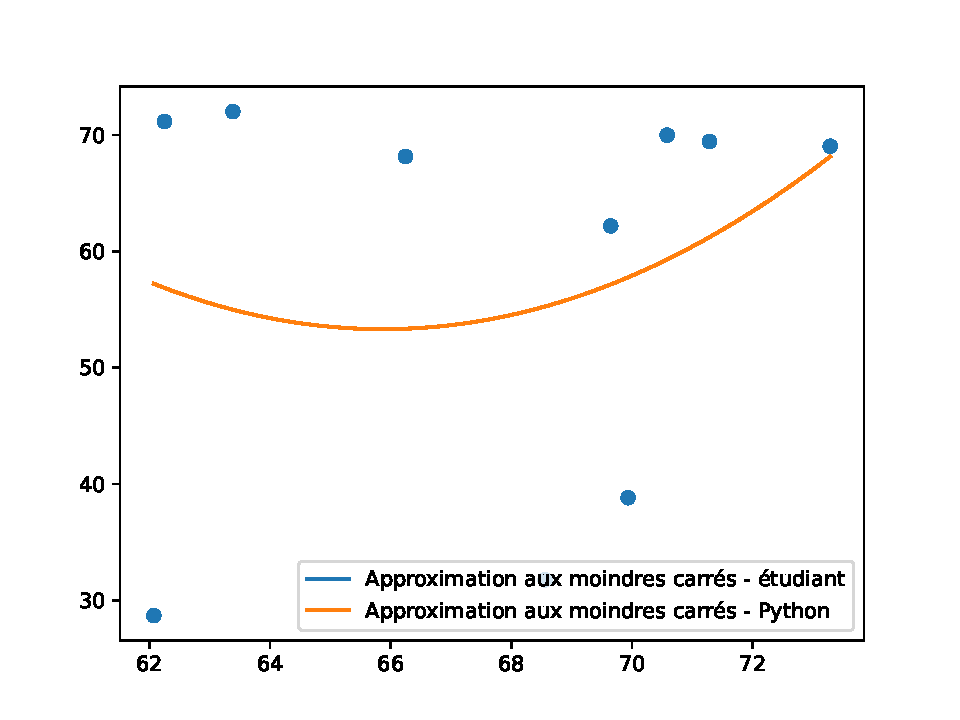
\includegraphics[width=\textwidth]{images/approximation.pdf}
    \end{center}
\end{figure}

\end{document}
